\section{Origine et concept}

Bien que le terme "pangénome" soit utilisé dans des articles avant 2005, en microbiologie, on s'accorde sur une origine du concept de pangénome proposé dans 2 articles fondateurs \cite{medini_microbial_2005,tettelin_genome_2005}.
L'idée est de ne pas représenter chaque génome individuellement, mais d'utiliser une structure mathématique permettant de les représenter tous simultanément.
Le pangénome représente l'union de toutes les séquences présentes dans un ensemble de génomes. En bioinformatique, la structure, les algorithmes, les méthodes d'analyses des pangénomes, ont constitué un nouveau champ de recherche, la pangénomique.

%\medskip

À partir du pangénome, Tettelin \textit{et al.} proposent de séparer les gènes en 2 catégories, les gènes "\textit{core}" communs à tous les génomes, des gènes "\textit{dispensable}" (ou \textit{accessory}) trouvés dans un sous-ensemble de génomes. En généralisant, le pangénome permet de distinguer l'ensemble des séquences communes à tous les organismes des variations présentes chez certains groupes d'individus, voire spécifiques à un organisme. De ce postulat a émergé l'idée de remplacer les génomes de référence dans les bases de données par des pangénomes de référence \cite{the_computational_pan-genomics_consortium_computational_2018}. Toutefois, ce changement de paradigme n'a pas encore été opéré, car aucune méthode n'a encore réussi à s'imposer comme solution optimale. Trouver une méthode globale est un défi, car la pangénomique est appliquée dans de nombreux domaines de recherche, pour répondre à une grande diversité de questions.

%\medskip

En 2018, le "Computational Pan-Genomics Consortium" met en avant le rôle de la pangénomique dans le développement de solutions applicatives répondant à des problématiques communes à plusieurs disciplines \cite{the_computational_pan-genomics_consortium_computational_2018}. En retour, la pangénomique bénéficie des avancées en phylogénie, métagénomique et intelligence artificielle.
En phylogénie, les méthodes de comparaison génomique à grande échelle et les techniques de construction d'arbres phylogénétiques ont été intégrées aux approches pangénomiques. Réciproquement, la pangénomique permet une meilleure prise en compte des variations génétiques à l'échelle de l'ensemble des génomes, plutôt que de se limiter à un génome de référence, offrant ainsi une vision plus fine de la dynamique évolutive \cite{bazinet_pan-genome_2017}.
Les données métagénomiques représentent un challenge pour la pangénomique. À partir des métagénomes, le pangénome doit être construit en étudiant les relations de co-occurrence des gènes, et non les relations évolutives. Ce changement représente un défi, notamment lorsque les lectures sont courtes. Toutefois, la pangénomique permet d'approfondir l’analyse de la diversité génétique des communautés microbiennes, et de mettre en évidence des adaptations communes à l'environnement ou des co-évolutions et des interactions entre les organismes \cite{the_computational_pan-genomics_consortium_computational_2018}.
L’intelligence artificielle joue également un rôle clé en améliorant l’annotation et la prédiction fonctionnelle des gènes. L’apprentissage automatique est appliqué à la pangénomique pour détecter des motifs génétiques pertinents, prédire des phénotypes et identifier des associations entre mutations et traits phénotypiques \cite{her_pan-genome-based_2018}. Ces méthodes, souvent développées pour d’autres disciplines, ont donc favorisé l’essor de la pangénomique en optimisant l’analyse des données, la reconstruction des génomes et l’interprétation des résultats.

%\medskip

La pangénomique représente une solution à l'analyse de grands volumes de données, à l'heure où le nombre de génomes disponibles dans les banques augmente de façon exponentielle. Entre 2006 et 2024, ce ne sont pas moins de 3 500 articles qui référencent le terme\footnote{Ce chiffre doit être revu à la baisse dû à l'utilisation erronée du terme dans certaines études et une utilisation parfois abusive pour profiter de l'intérêt croissant pour ces analyses}, dont près de 800 concernant les procaryotes (\autoref{fig:panCite}).

\begin{figure}[htbp]
    \centering
    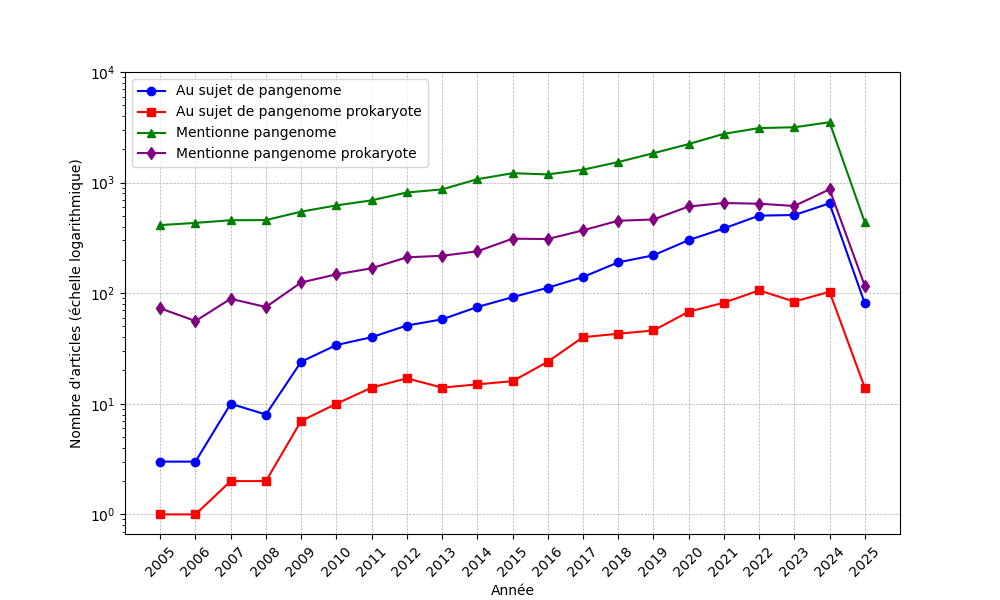
\includegraphics[width=\linewidth]{images/pangenomeCitation.png}
    \caption[Bibliométrie pangénome]{\textbf{Nombre d'articles, référencés dans PubMed, par année, à propos de pangénome du 1er janvier 2004 au 10 février 2025}. La courbe bleue représente le nombre d'articles contenant le terme pangénome dans le titre ou l'abstract : Query=("pan-genome"[Title/Abstract] OR "pangenome"[Title/Abstract] OR "pan-genome"[Title/Abstract]) AND (2004:2025[pdat]). La courbe rouge limite aux publications concernant les procaryotes : Query=("procaryote"[Title/Abstract] OR "bacteria"[Title/Abstract] OR "archeae"[Title/Abstract]) AND ("pan-genome"[Title/Abstract] OR "pangenome"[Title/Abstract] OR "pan-genome"[Title/Abstract]) AND (2004:2025[pdat]). La courbe verte représente tous les articles ou le terme pangénome est trouvé : Query=((pangenome) OR (pan genome)) OR (pan-genome) AND (2004:2025[pdat]). La courbe violette filtre les publications concernant les procaryotes : Query=(((procaryote) OR (bacteria)) OR (archeae)) AND (((pan-genome) OR (pangenome)) OR (pan genome)) AND (2004:2025[pdat]).}
    \label{fig:panCite}
\end{figure}

\newpage
\subsection{Modélisation de la croissance des pangénomes}
\label{sec:croissance_pan}

Dans l'article original de Tettelin \textit{et al.} \cite{tettelin_genome_2005}, les auteurs se sont intéressés à la distribution \textit{core/dispensable} en fonction du nombre de génomes de \textit{Streptococcus agalactiae}\footnote{Bactérie du microbiote intestinale humain et animal, qui est également associé à des infections graves.} que contient le pangénome. Ils observent que lorsque le nombre de génomes augmente, la part de \textit{core genome} décroît de façon exponentielle. Ce résultat les amène à modéliser la croissance du \textit{core genomes} selon une équation exponentielle décroissante. Le modèle permet alors d'estimer la taille du \textit{core genome} pour un nombre de génomes en théorie infinie. Il est alors possible d'estimer la taille du \textit{core genome} d'une espèce à partir d'un échantillon de génome. 

À partir de ce modèle, il est également possible d'estimer la taille du pangénome, \textit{i.e.}, le nombre de gènes unique que contient le pangénome. Ils définissent alors 2 types de pangénomes en fonction de l'estimation de la taille : les \textbf{pangénomes ouverts} et les \textbf{pangénomes fermés}. Les pangénomes sont considérés comme ouverts lorsque l'on ajoute un génome, le nombre de gènes ajouté au pangénome augmentent. Le nombre de gènes est donc théoriquement infini pour un pangénome ouvert avec une infinité de génomes. Les pangénomes fermés quant à eux voient le nombre de nouveaux gènes progressivement diminuer lors de l'ajout de nouveaux génomes. La courbe de prédiction permet d'identifier un plateau théorique du nombre maximal de familles que contiendra le pangénome avec un nombre de génomes infinis. Biologiquement, le pangénome ouvert est attendu pour les espèces sympatriques\footnote{Espèces vivant dans le même environnement que d'autres espèces.} et qui présentent un fort taux de transferts horizontaux, tandis que les espèces vivant dans des niches écologiques ou qui ont une faible capacité d'acquisition de gènes extérieurs vont avoir un pangénome fermé.

\begin{figure}[htbp]
    \centering
    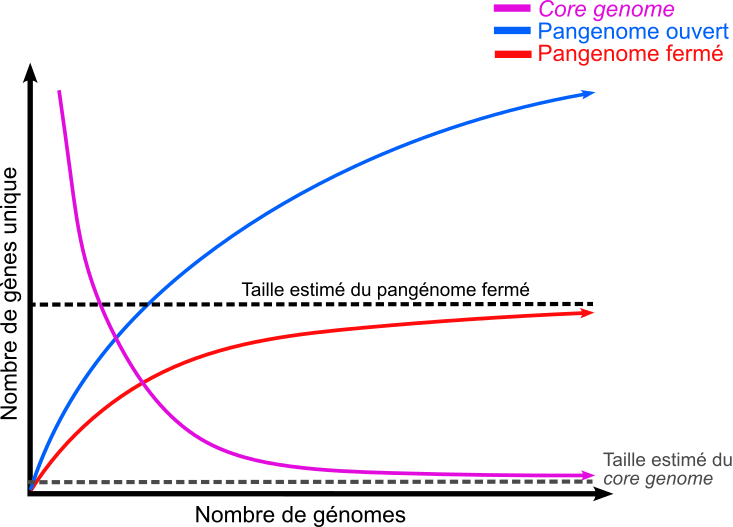
\includegraphics[width=0.85\linewidth]{images/panOpenClose.png}
    \caption[Schéma de croissance du pangénome]{\textbf{Schéma de croissance du pangénome.}}
    \label{fig:panOpenClose}
\end{figure}

Le modèle proposé par Tettelin \textit{et al.}, repose sur l'hypothèse que pour un nombre suffisant de génomes, le nombre de nouveaux gènes apportés par un génome devient constant à partir d'un certain nombre de génomes \cite{tettelin_genome_2005}. Cette hypothèse implique alors que la taille du pangénome est infinie. Cette hypothèse sera questionnée par Hogg \textit{et al.} dans leur étude du pangénome de \textit{Haemophilus influenzae} \cite{hogg_characterization_2007}. Ils vont alors proposer une modélisation basée sur l'hypothèse que le pangénome est fini. Dans leur modèle, chaque gène est associé à une variable aléatoire de Bernoulli, dont la probabilité correspond à la fréquence du gène dans les génomes. Un génome est ainsi généré en observant ces variables : un gène est présent si l’essai est un succès, sinon il est absent. Bien que certains gènes ne soient pas indépendants en raison de structures comme les îlots génomiques, cette hypothèse est conservée pour simplifier le modèle. Les fréquences réelles des gènes étant inconnues, elles sont modélisées de manière probabiliste en répartissant les gènes en $K$ classes distinctes, chacune ayant une fréquence de présence spécifique. À partir de ce modèle, sur le pangénome de \textit{H. influenzae} avec $K=7$, la taille du pangénome est estimée à 5 000 gènes (contre 2 800 gènes dans les 13 génomes de base). Ce modèle sera ensuite amélioré par Snipen \textit{et al.} \cite{snipen_microbial_2009}, qui proposeront une détermination automatique du nombre de classes $K$ et de la fréquence théorique des gènes pour chaque classe. Les modèles binomiaux proposent une perspective dans laquelle la diversité en gènes est finie et qu'il existe un nombre de génomes suffisamment grand pour que tout le répertoire génique soit connu. Cette vision semble de prime abord logique, car le nombre de combinaisons possibles de nucléotides ou d'acides aminés est fini. Pourtant, on peut y opposer que ce nombre, sans le calculer, semble démesuré et qu'il peut être considéré comme infini. De plus, les génomes évoluent continuellement et de nouveaux gènes apparaissent sans cesse. L'utilisation des modèles binomiaux semble alors plus appropriée à des espèces de niche, isolées et présentant un faible taux de transferts horizontaux.

En 2008, Tettelin \textit{et al.} vont proposer une nouvelle modélisation basée sur la loi de Heaps\footnote{Définit de manière empirique en linguistique, cette loi permet de décrire le nombre de mots d'une langue à partir d'un ensemble de documents.} \cite{tettelin_comparative_2008}. On estime le nombre $n$ de gènes distincts, en fonction du nombre $N$ de génomes étudiés, selon la relation :
\begin{equation}
    n=kN^\gamma, 0<\gamma<1,k\geq1
\end{equation}

Le paramètre $k$ est une constante de proportionnalité tandis que $\gamma$ reflète la tendance de la fonction. Ainsi, plus $\gamma$ est proche de 0 plus la croissance en gènes distincts est lente, et plus $\gamma$ est proche de 1 plus la croissance est rapide (\autoref{fig:HeaplawGamma}).

\begin{figure}[htbp]
    \centering
    \subfloat[Courbe de croissance selon la loi de Heap]{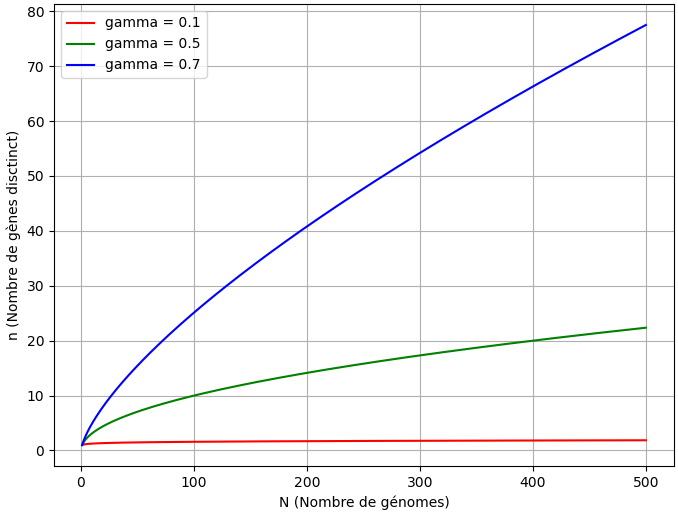
\includegraphics[width=0.48\linewidth]{images/HeapsLawgamma.png}
    \label{fig:HeaplawGamma}}
    \hfill
    \subfloat[Courbe de raréfaction selon la loi de Heap]{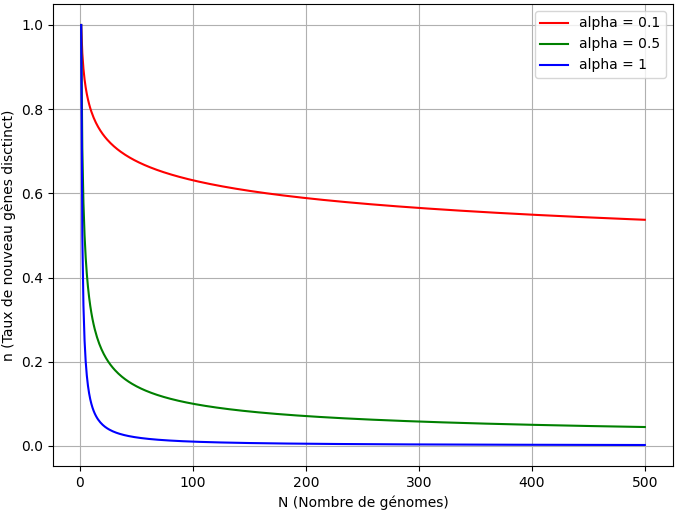
\includegraphics[width=0.48\linewidth]{images/HeapsLawAlpha.png}
    \label{fig:HeaplawAlpha}}
    \caption[Évolution du pangénome : visualisation de la croissance et de la raréfaction du contenue génique selon la loi de Heap]{\textbf{Évolution du pangénome : visualisation de la croissance et de la raréfaction du contenue génique selon la loi de Heap.}}
    \label{fig:Heaplaw}
\end{figure}

Selon la loi de Heap, le nombre de nouveaux gènes découverts diminue à mesure que l'on ajoute des génomes. On peut formuler ceci selon l'équation : 

\begin{equation}
    p(n)=kN^{(\gamma-1)}=kN^{-\alpha}, \alpha=1-\gamma
\end{equation}

Ainsi, sur la \autoref{fig:HeaplawAlpha}, lorsque $0<\alpha<1$, le taux de nouveaux gènes décroît en ajoutant des génomes, sans jamais être nul. Dans ce cas, le nombre de gènes distincts est croissant. Ce qui implique que si $0<\alpha<1$, le pangénome est ouvert. À partir d'un ensemble de génomes, il est possible d'estimer k et $\alpha$ (ou $\gamma$) et donc de caractériser si le pangénome est ouvert. Si $\alpha\geq1$, alors le taux de nouveaux gènes atteint 0, ce qui correspond à un pangénome fermé. 

\newpage

\subsection{Les différents types de pangénomes}

Les pangénomes peuvent être divisés en 2 catégories en fonction de l'unité choisie pour les construire. Le premier type, celui présenté par Tettelin \textit{et al.} \cite{tettelin_genome_2005}, utilise les gènes comme unité de base du pangénome (\autoref{fig:panType}.B). En regroupant les gènes par homologie (appelé famille de gènes, cf. \autoref{sec:clustering}), il est possible d'obtenir la présence/absence de gènes similaires dans les génomes. Ces pangénomes ont l'avantage d'être moins coûteux en ressources de calcul pour être construits. De plus, ils sont faciles à interpréter, car les gènes sont des unités déjà bien définies et parfois, ils sont même annotés fonctionnellement. Néanmoins, en utilisant les gènes, la méthode d'annotation a un impact important sur le pangénome et il est sensible aux erreurs d'annotation. De plus, les régions non codantes ne sont pas prises en compte dans cette approche. Enfin, les SNPs peuvent passer inaperçus après le regroupement, ainsi que les variants structuraux (SV).

L'autre type de pangénome est basé sur les séquences brutes des génomes. Bien que le terme pangénome n’ait pas encore été employé à l’époque, Chiapello \textit{et al.} \cite{chiapello_systematic_2005} ont proposé une méthode de segmentation des génomes en deux composantes : la "colonne vertébrale", représentant les régions conservées, et les "boucles", qui correspondent aux parties variables. Plus tard, l’outil GenomeMapper \cite{schneeberger_simultaneous_2009}, a explicitement introduit la notion de pangénome de séquence. Son approche repose sur un alignement global des séquences, analysées à travers des k-mers pour différencier les segments conservés des segments variables (\autoref{fig:panType}.C,D). Cette approche a l'intérêt de prendre en compte toute la diversité des génomes (codant, non codant, SNPs et SV). Toutefois, la construction de ces pangénomes est plus coûteuse en ressources. De plus, l'interprétation est plus complexe, car le pangénome n'est pas annoté au départ. Pour terminer, certaines méthodes de construction, utilisent un génome de référence comme séquence de base (\autoref{fig:panType}.C), ce qui peut aussi introduire un biais.

\begin{figure}[htbp]
    \centering
    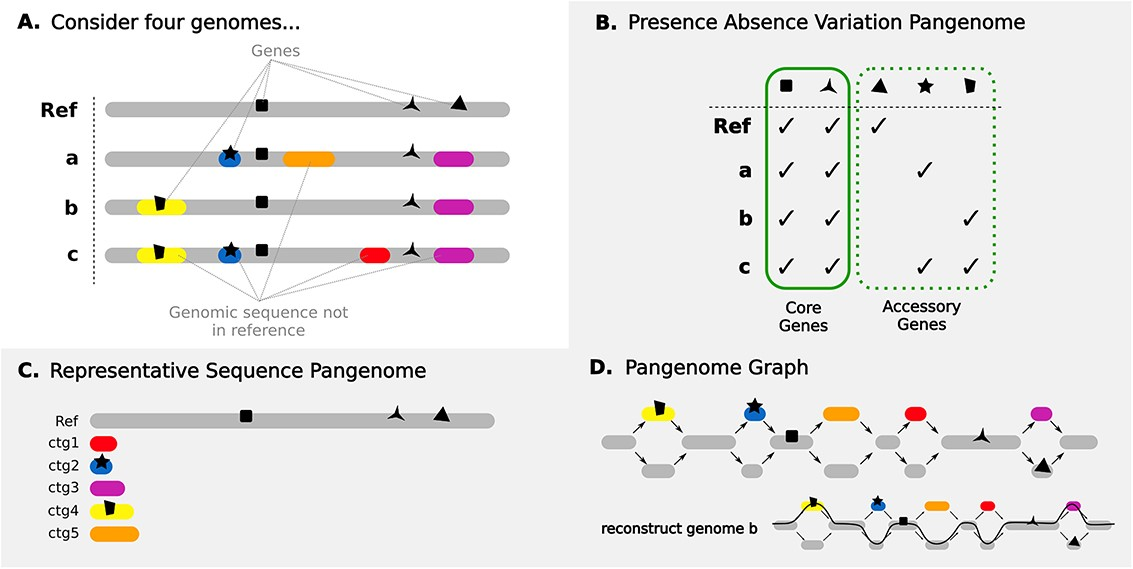
\includegraphics[width=0.8\linewidth]{images/pangenomeTypes.jpeg}
    \caption[Différents types de pangénomes]{\textbf{Différents types de pangénomes.} Extrait de \cite{matthews_gentle_2024}}
    \label{fig:panType}
\end{figure}
